\documentclass{standalone}
\usepackage{tikz}
\usetikzlibrary{patterns, positioning}

\begin{document}
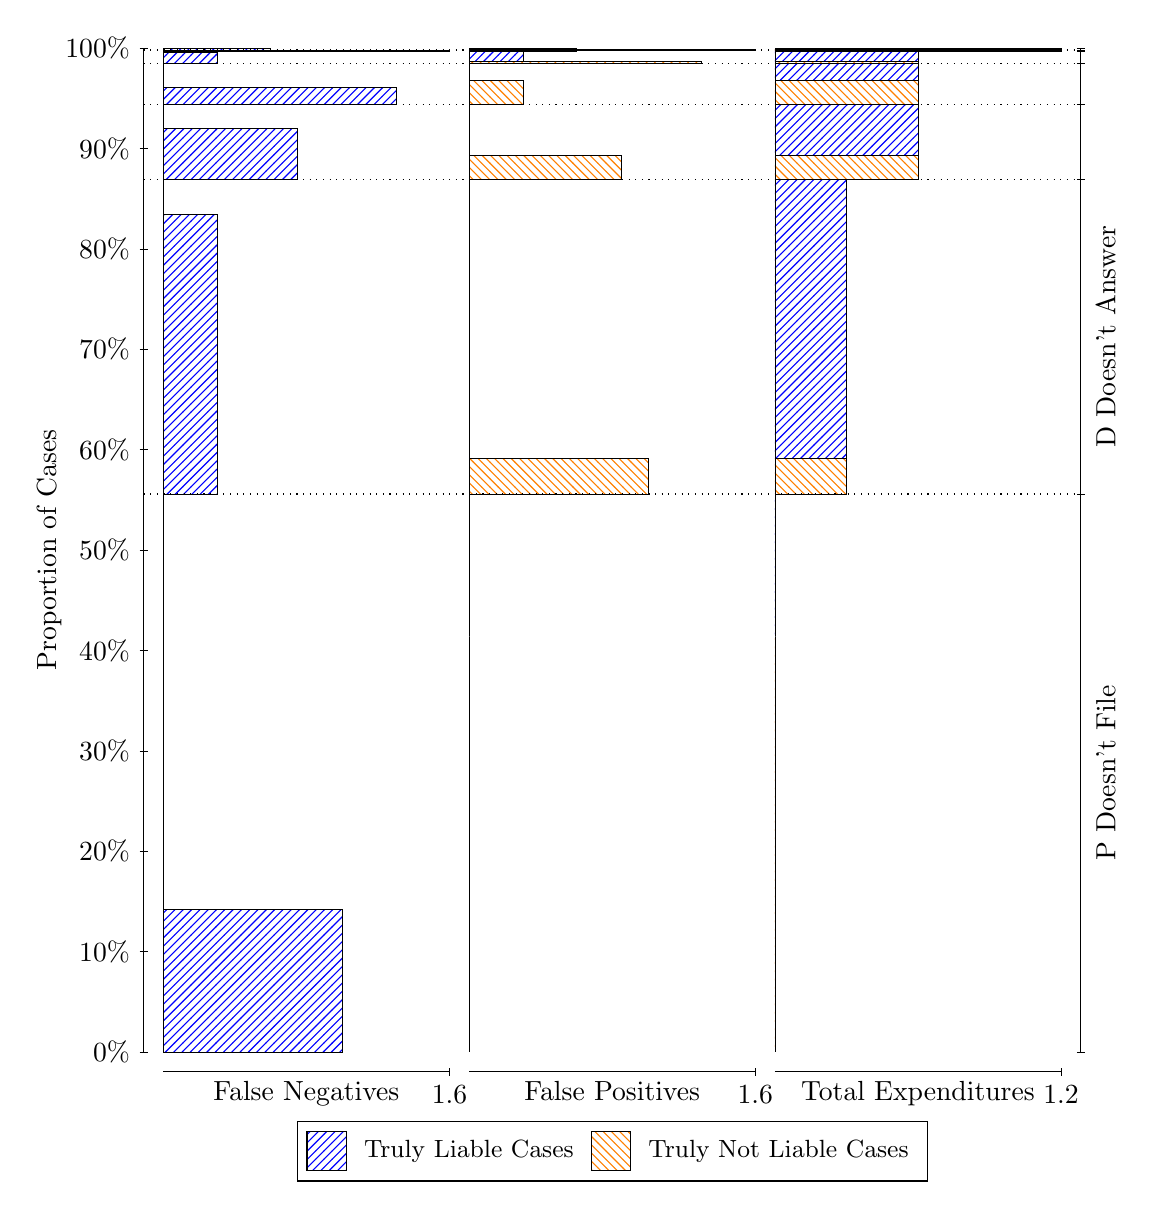
\begin{tikzpicture}
\draw[black, very thin] (1.5,1.75) -- (1.5,14.5);
\node[rotate=90, anchor=center] at (0.3, 8.125) {Proportion of Cases};
\draw[black, very thin] (1.45,1.75) -- (1.55,1.75);
\node[anchor=east] at (1.45, 1.75) {0\%};
\draw[black, very thin] (1.45,3.025) -- (1.55,3.025);
\node[anchor=east] at (1.45, 3.025) {10\%};
\draw[black, very thin] (1.45,4.3) -- (1.55,4.3);
\node[anchor=east] at (1.45, 4.3) {20\%};
\draw[black, very thin] (1.45,5.575) -- (1.55,5.575);
\node[anchor=east] at (1.45, 5.575) {30\%};
\draw[black, very thin] (1.45,6.85) -- (1.55,6.85);
\node[anchor=east] at (1.45, 6.85) {40\%};
\draw[black, very thin] (1.45,8.125) -- (1.55,8.125);
\node[anchor=east] at (1.45, 8.125) {50\%};
\draw[black, very thin] (1.45,9.4) -- (1.55,9.4);
\node[anchor=east] at (1.45, 9.4) {60\%};
\draw[black, very thin] (1.45,10.675) -- (1.55,10.675);
\node[anchor=east] at (1.45, 10.675) {70\%};
\draw[black, very thin] (1.45,11.95) -- (1.55,11.95);
\node[anchor=east] at (1.45, 11.95) {80\%};
\draw[black, very thin] (1.45,13.225) -- (1.55,13.225);
\node[anchor=east] at (1.45, 13.225) {90\%};
\draw[black, very thin] (1.45,14.5) -- (1.55,14.5);
\node[anchor=east] at (1.45, 14.5) {100\%};

\draw[black, very thin] (13.4,1.75) -- (13.4,14.5);
\draw[black, very thin] (13.35,1.75) -- (13.45,1.75);
\node[anchor=west] at (13.35, 1.75) {};
\draw[black, very thin] (13.35,8.8359) -- (13.45,8.8359);
\node[anchor=west] at (13.35, 8.8359) {};
\draw[black, very thin] (13.35,12.833) -- (13.45,12.833);
\node[anchor=west] at (13.35, 12.833) {};
\draw[black, very thin] (13.35,13.784) -- (13.45,13.784);
\node[anchor=west] at (13.35, 13.784) {};
\draw[black, very thin] (13.35,14.309) -- (13.45,14.309);
\node[anchor=west] at (13.35, 14.309) {};
\draw[black, very thin] (13.35,14.465) -- (13.45,14.465);
\node[anchor=west] at (13.35, 14.465) {};
\draw[black, very thin] (13.35,14.475) -- (13.45,14.475);
\node[anchor=west] at (13.35, 14.475) {};
\draw[black, very thin] (13.35,14.5) -- (13.45,14.5);
\node[anchor=west] at (13.35, 14.5) {};

\draw[black, very thin, pattern color=blue, pattern=north east lines] (1.75,1.75) rectangle (4.0208,3.5573);
\draw[black, very thin, pattern color=orange, pattern=north west lines] (1.75,3.5573) rectangle (1.75,8.8359);
\draw[black, very thin, pattern color=blue, pattern=north east lines] (1.75,8.8359) rectangle (2.4312,12.384);
\draw[black, very thin, pattern color=orange, pattern=north west lines] (1.75,12.384) rectangle (1.75,12.833);
\draw[black, very thin, pattern color=blue, pattern=north east lines] (1.75,12.833) rectangle (3.4531,13.476);
\draw[black, very thin, pattern color=orange, pattern=north west lines] (1.75,13.476) rectangle (1.75,13.784);
\draw[black, very thin, pattern color=blue, pattern=north east lines] (1.75,13.784) rectangle (4.7021,14.003);
\draw[black, very thin, pattern color=orange, pattern=north west lines] (1.75,14.003) rectangle (1.75,14.309);
\draw[black, very thin, pattern color=blue, pattern=north east lines] (1.75,14.309) rectangle (2.4312,14.442);
\draw[black, very thin, pattern color=orange, pattern=north west lines] (1.75,14.442) rectangle (1.75,14.465);
\draw[black, very thin, pattern color=blue, pattern=north east lines] (1.75,14.465) rectangle (5.3833,14.471);
\draw[black, very thin, pattern color=orange, pattern=north west lines] (1.75,14.471) rectangle (1.75,14.475);
\draw[black, very thin, pattern color=blue, pattern=north east lines] (1.75,14.475) rectangle (3.1125,14.495);
\draw[black, very thin, pattern color=orange, pattern=north west lines] (1.75,14.495) rectangle (1.75,14.5);
\draw[black, very thin, pattern color=orange, pattern=north west lines] (5.6333,1.75) rectangle (5.6333,7.0286);
\draw[black, very thin, pattern color=blue, pattern=north east lines] (5.6333,7.0286) rectangle (5.6333,8.8359);
\draw[black, very thin, pattern color=orange, pattern=north west lines] (5.6333,8.8359) rectangle (7.9042,9.285);
\draw[black, very thin, pattern color=blue, pattern=north east lines] (5.6333,9.285) rectangle (5.6333,12.833);
\draw[black, very thin, pattern color=orange, pattern=north west lines] (5.6333,12.833) rectangle (7.5635,13.141);
\draw[black, very thin, pattern color=blue, pattern=north east lines] (5.6333,13.141) rectangle (5.6333,13.784);
\draw[black, very thin, pattern color=orange, pattern=north west lines] (5.6333,13.784) rectangle (6.3146,14.09);
\draw[black, very thin, pattern color=blue, pattern=north east lines] (5.6333,14.09) rectangle (5.6333,14.309);
\draw[black, very thin, pattern color=orange, pattern=north west lines] (5.6333,14.309) rectangle (8.5854,14.332);
\draw[black, very thin, pattern color=blue, pattern=north east lines] (5.6333,14.332) rectangle (6.3146,14.465);
\draw[black, very thin, pattern color=orange, pattern=north west lines] (5.6333,14.465) rectangle (6.9958,14.47);
\draw[black, very thin, pattern color=blue, pattern=north east lines] (5.6333,14.47) rectangle (5.6333,14.475);
\draw[black, very thin, pattern color=orange, pattern=north west lines] (5.6333,14.475) rectangle (9.2667,14.481);
\draw[black, very thin, pattern color=blue, pattern=north east lines] (5.6333,14.481) rectangle (6.9958,14.5);
\draw[black, very thin, pattern color=orange, pattern=north west lines] (9.5167,1.75) rectangle (9.5167,7.0286);
\draw[black, very thin, pattern color=blue, pattern=north east lines] (9.5167,7.0286) rectangle (9.5167,8.8359);
\draw[black, very thin, pattern color=orange, pattern=north west lines] (9.5167,8.8359) rectangle (10.425,9.285);
\draw[black, very thin, pattern color=blue, pattern=north east lines] (9.5167,9.285) rectangle (10.425,12.833);
\draw[black, very thin, pattern color=orange, pattern=north west lines] (9.5167,12.833) rectangle (11.333,13.141);
\draw[black, very thin, pattern color=blue, pattern=north east lines] (9.5167,13.141) rectangle (11.333,13.784);
\draw[black, very thin, pattern color=orange, pattern=north west lines] (9.5167,13.784) rectangle (11.333,14.09);
\draw[black, very thin, pattern color=blue, pattern=north east lines] (9.5167,14.09) rectangle (11.333,14.309);
\draw[black, very thin, pattern color=orange, pattern=north west lines] (9.5167,14.309) rectangle (11.333,14.332);
\draw[black, very thin, pattern color=blue, pattern=north east lines] (9.5167,14.332) rectangle (11.333,14.465);
\draw[black, very thin, pattern color=orange, pattern=north west lines] (9.5167,14.465) rectangle (13.15,14.47);
\draw[black, very thin, pattern color=blue, pattern=north east lines] (9.5167,14.47) rectangle (13.15,14.475);
\draw[black, very thin, pattern color=orange, pattern=north west lines] (9.5167,14.475) rectangle (13.15,14.481);
\draw[black, very thin, pattern color=blue, pattern=north east lines] (9.5167,14.481) rectangle (13.15,14.5);
\draw[black, dotted] (1.5,8.8359) -- (13.4,8.8359);
\draw[black, dotted] (1.5,12.833) -- (13.4,12.833);
\draw[black, dotted] (1.5,13.784) -- (13.4,13.784);
\draw[black, dotted] (1.5,14.309) -- (13.4,14.309);
\draw[black, dotted] (1.5,14.465) -- (13.4,14.465);
\draw[black, dotted] (1.5,14.475) -- (13.4,14.475);
\draw[black, very thin] (1.75,1.5) -- (5.3833,1.5);
\node[anchor=north] at (3.5667, 1.5) {False Negatives};
\draw[black, very thin] (5.3833,1.45) -- (5.3833,1.55);
\node[anchor=north] at (5.3833, 1.45) {1.6};

\draw[black, very thin] (5.6333,1.5) -- (9.2667,1.5);
\node[anchor=north] at (7.45, 1.5) {False Positives};
\draw[black, very thin] (9.2667,1.45) -- (9.2667,1.55);
\node[anchor=north] at (9.2667, 1.45) {1.6};

\draw[black, very thin] (9.5167,1.5) -- (13.15,1.5);
\node[anchor=north] at (11.333, 1.5) {Total Expenditures};
\draw[black, very thin] (13.15,1.45) -- (13.15,1.55);
\node[anchor=north] at (13.15, 1.45) {1.2};

\node[black, centered, rotate=90] at (13.72, 5.293) {P Doesn't File};
\node[black, centered, rotate=90] at (13.72, 10.834) {D Doesn't Answer};






\draw (7.449999999999999,1.5) node[draw=none] (baseCoordinate) {};
\begin{scope}[align=center]
        \matrix[scale=0.5, draw=black, below=0.5cm of baseCoordinate, nodes={draw}, column sep=0.1cm]{
            \node[rectangle, draw, minimum width=0.5cm, minimum height=0.5cm, pattern=north east lines, pattern color=blue] {}; &
            \node[draw=none, font=\small] (B) {Truly Liable Cases}; &
            \node[rectangle, draw, minimum width=0.5cm, minimum height=0.5cm, pattern=north west lines, pattern color=orange] {}; &
            \node[draw=none, font=\small] (B) {Truly Not Liable Cases}; \\
            };
\end{scope}

\end{tikzpicture}
\end{document}